\section{PVPhysics Class Reference}
\label{class_p_v_physics}\index{PVPhysics@{PVPhysics}}
Collaboration diagram for PVPhysics:\nopagebreak
\begin{figure}[H]
\begin{center}
\leavevmode
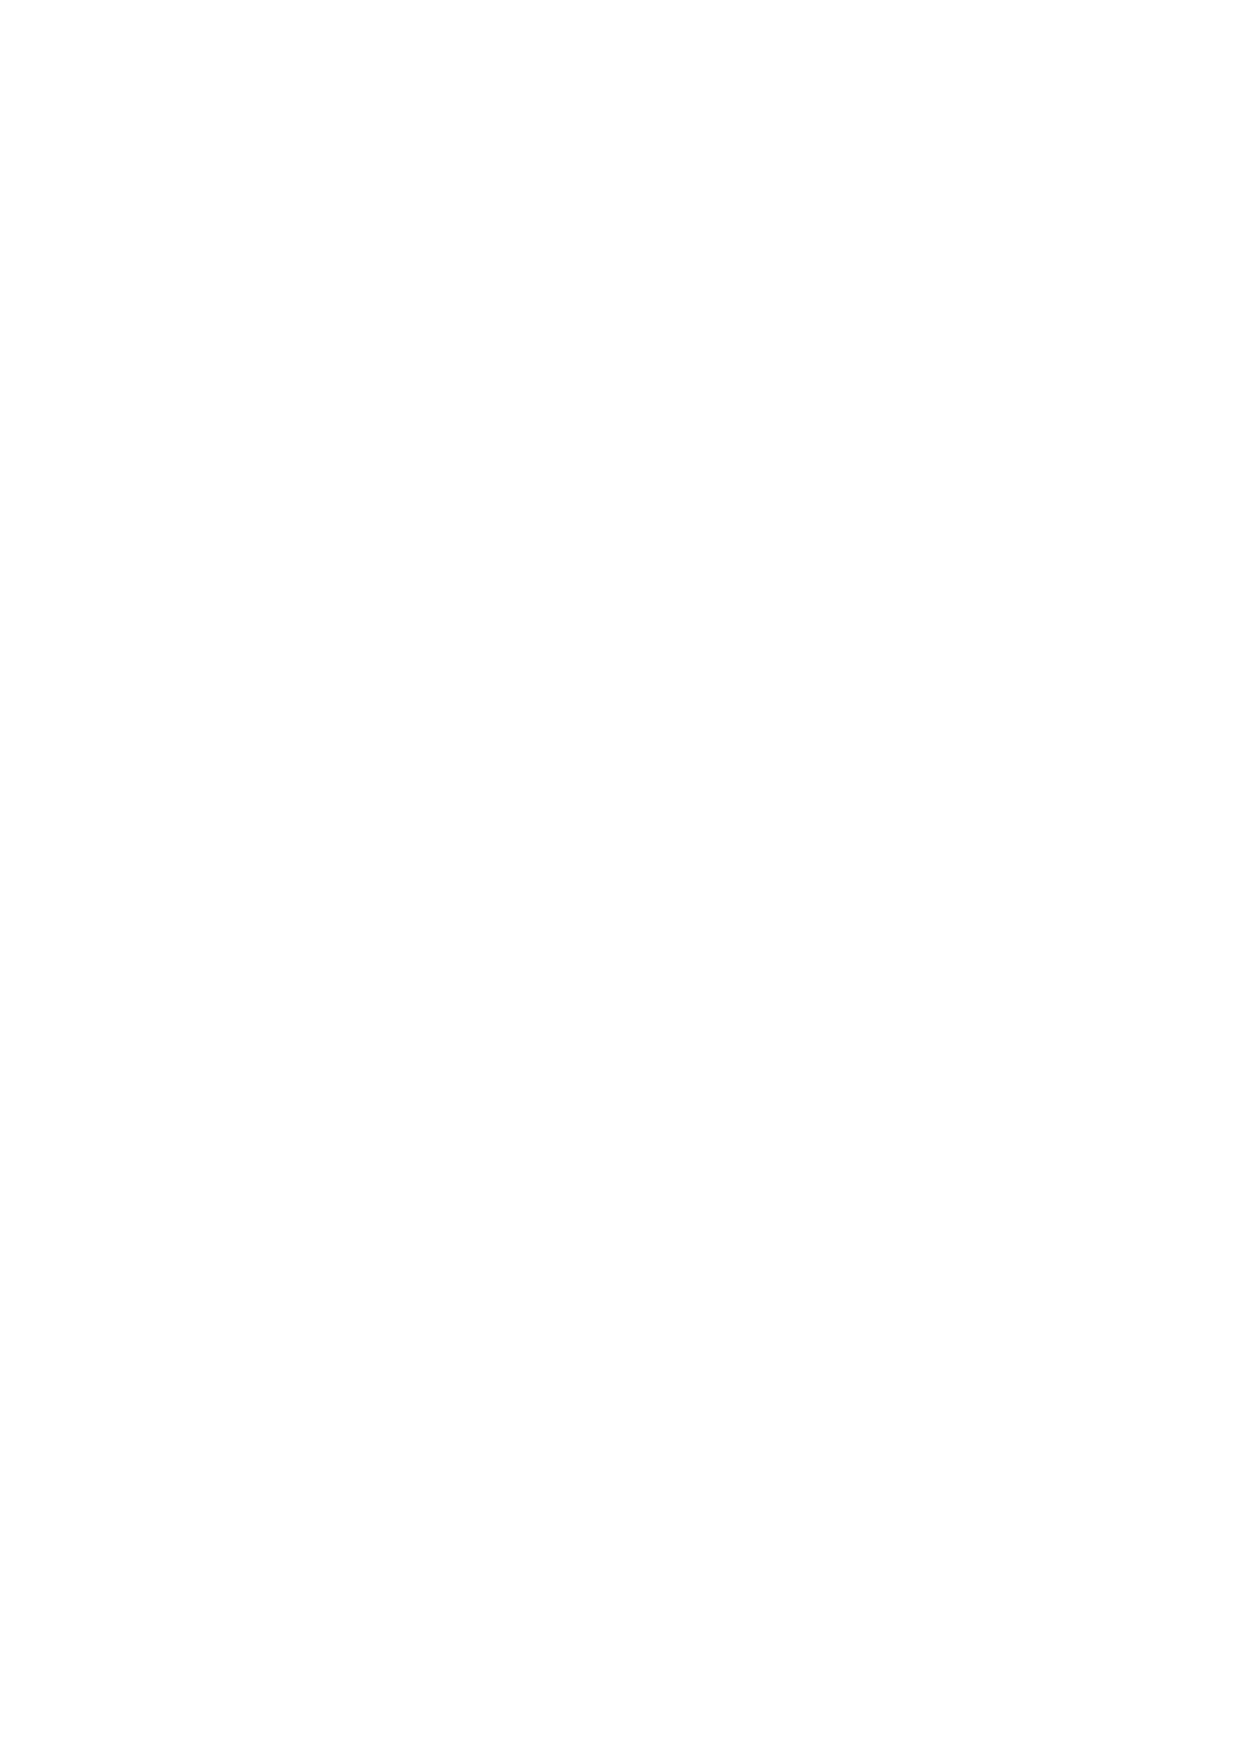
\includegraphics[width=44pt]{class_p_v_physics__coll__graph}
\end{center}
\end{figure}
\subsection*{Public Member Functions}
\begin{CompactItemize}
\item 
{\bf PVPhysics} ()
\item 
{\bf $\sim$PVPhysics} ()
\item 
void {\bf simulate} (std::map$<$ std::string, {\bf PVNode} $\ast$ $>$ \&objectMap, std::vector$<$ {\bf PVNode} $\ast$ $>$ \&balls, int numberOfFlyingBalls, float time)
\item 
void {\bf move} ({\bf PVNode} $\ast$ball, float time)
\item 
void {\bf collisionDetection} (std::map$<$ std::string, {\bf PVNode} $\ast$ $>$ \&objectMap, std::vector$<$ {\bf PVNode} $\ast$ $>$ \&balls, int numberOfFlyingBalls)
\item 
void {\bf collisionWithArena} ({\bf PVNode} $\ast$arena, {\bf PVNode} $\ast$ball)
\item 
void {\bf collisionWithWall} ({\bf PVNode} $\ast$wall, {\bf PVNode} $\ast$ball)
\item 
void {\bf collisionWithCannon} ({\bf PVNode} $\ast$kanone, {\bf PVNode} $\ast$ball)
\item 
void {\bf collisionWithBall} ({\bf PVNode} $\ast$ball1, {\bf PVNode} $\ast$ball2)
\item 
void {\bf collisionWithPillar} ({\bf PVNode} $\ast$pillar, {\bf PVNode} $\ast$ball)
\item 
void {\bf handleCollision} ({\bf PVNode} $\ast$node, {\bf PVNode} $\ast$ball)
\item 
void {\bf handleCollisionWithGround} ({\bf PVNode} $\ast$ground, {\bf PVNode} $\ast$ball)
\item 
void {\bf handleCollisionWithBall} ({\bf PVNode} $\ast$ball1, {\bf PVNode} $\ast$ball2)
\end{CompactItemize}


\subsection{Constructor \& Destructor Documentation}
\index{PVPhysics@{PVPhysics}!PVPhysics@{PVPhysics}}
\index{PVPhysics@{PVPhysics}!PVPhysics@{PVPhysics}}
\subsubsection[{PVPhysics}]{\setlength{\rightskip}{0pt plus 5cm}PVPhysics::PVPhysics ()}\label{class_p_v_physics_aed6e907849a824d51cc2ddd1ab946d7}


Constructor. 

\index{PVPhysics@{PVPhysics}!$\sim$PVPhysics@{$\sim$PVPhysics}}
\index{$\sim$PVPhysics@{$\sim$PVPhysics}!PVPhysics@{PVPhysics}}
\subsubsection[{$\sim$PVPhysics}]{\setlength{\rightskip}{0pt plus 5cm}PVPhysics::$\sim$PVPhysics ()}\label{class_p_v_physics_d1b6443d26383106cb3322671974d48e}


Destructor. 



\subsection{Member Function Documentation}
\index{PVPhysics@{PVPhysics}!simulate@{simulate}}
\index{simulate@{simulate}!PVPhysics@{PVPhysics}}
\subsubsection[{simulate}]{\setlength{\rightskip}{0pt plus 5cm}void PVPhysics::simulate (std::map$<$ std::string, {\bf PVNode} $\ast$ $>$ \& {\em objectMap}, \/  std::vector$<$ {\bf PVNode} $\ast$ $>$ \& {\em balls}, \/  int {\em numberOfFlyingBalls}, \/  float {\em time})}\label{class_p_v_physics_d12e7af8e342acdf42f83d5f1e88dc14}


simulate function which calls move function and collision detection. 

\begin{Desc}
\item[Parameters:]
\begin{description}
\item[{\em objectMap}]map with objects. \item[{\em numberOfFlyingBalls}]current sooted balls. \item[{\em time}]delta time elapsed since last frame in seconds. \end{description}
\end{Desc}
\index{PVPhysics@{PVPhysics}!move@{move}}
\index{move@{move}!PVPhysics@{PVPhysics}}
\subsubsection[{move}]{\setlength{\rightskip}{0pt plus 5cm}void PVPhysics::move ({\bf PVNode} $\ast$ {\em ball}, \/  float {\em time})}\label{class_p_v_physics_ef493f065afc2637f704ec9fd5cb8754}


function for shooting a ball. 

\begin{Desc}
\item[Parameters:]
\begin{description}
\item[{\em ball}]a PVnode. \item[{\em time}]a float for the time since last frame. \end{description}
\end{Desc}
\index{PVPhysics@{PVPhysics}!collisionDetection@{collisionDetection}}
\index{collisionDetection@{collisionDetection}!PVPhysics@{PVPhysics}}
\subsubsection[{collisionDetection}]{\setlength{\rightskip}{0pt plus 5cm}void PVPhysics::collisionDetection (std::map$<$ std::string, {\bf PVNode} $\ast$ $>$ \& {\em objectMap}, \/  std::vector$<$ {\bf PVNode} $\ast$ $>$ \& {\em balls}, \/  int {\em numberOfFlyingBalls})}\label{class_p_v_physics_e56c458a7f62c983e2ab5f903bee9478}


function for calling the particular collision detection function for each node type. 

\begin{Desc}
\item[Parameters:]
\begin{description}
\item[{\em objectMap}]map with all scene nodes. \item[{\em balls}]vector with all balls. \end{description}
\end{Desc}
\index{PVPhysics@{PVPhysics}!collisionWithArena@{collisionWithArena}}
\index{collisionWithArena@{collisionWithArena}!PVPhysics@{PVPhysics}}
\subsubsection[{collisionWithArena}]{\setlength{\rightskip}{0pt plus 5cm}void PVPhysics::collisionWithArena ({\bf PVNode} $\ast$ {\em arena}, \/  {\bf PVNode} $\ast$ {\em ball})}\label{class_p_v_physics_35f87bc90c8aae2772d79523bcb4bf77}


detects collision between arena and a ball. 

\begin{Desc}
\item[Parameters:]
\begin{description}
\item[{\em $\ast$arena}]scene node. \item[{\em $\ast$ball}]\end{description}
\end{Desc}
\index{PVPhysics@{PVPhysics}!collisionWithWall@{collisionWithWall}}
\index{collisionWithWall@{collisionWithWall}!PVPhysics@{PVPhysics}}
\subsubsection[{collisionWithWall}]{\setlength{\rightskip}{0pt plus 5cm}void PVPhysics::collisionWithWall ({\bf PVNode} $\ast$ {\em wall}, \/  {\bf PVNode} $\ast$ {\em ball})}\label{class_p_v_physics_7e07bd0171a431a2ccf4e542348d0820}


detects collision between wall and a ball. 

\begin{Desc}
\item[Parameters:]
\begin{description}
\item[{\em $\ast$wall}]scene node. \item[{\em $\ast$ball}]\end{description}
\end{Desc}
\index{PVPhysics@{PVPhysics}!collisionWithCannon@{collisionWithCannon}}
\index{collisionWithCannon@{collisionWithCannon}!PVPhysics@{PVPhysics}}
\subsubsection[{collisionWithCannon}]{\setlength{\rightskip}{0pt plus 5cm}void PVPhysics::collisionWithCannon ({\bf PVNode} $\ast$ {\em kanone}, \/  {\bf PVNode} $\ast$ {\em ball})}\label{class_p_v_physics_967d8b19b11aef754591e6d9336ecfbe}


detects collision between arena and a ball. 

\begin{Desc}
\item[Parameters:]
\begin{description}
\item[{\em $\ast$kanone}]scene node \item[{\em $\ast$ball}]\end{description}
\end{Desc}
\index{PVPhysics@{PVPhysics}!collisionWithBall@{collisionWithBall}}
\index{collisionWithBall@{collisionWithBall}!PVPhysics@{PVPhysics}}
\subsubsection[{collisionWithBall}]{\setlength{\rightskip}{0pt plus 5cm}void PVPhysics::collisionWithBall ({\bf PVNode} $\ast$ {\em ball1}, \/  {\bf PVNode} $\ast$ {\em ball2})}\label{class_p_v_physics_d55e28ab26fc818faf43231a3368294c}


detects collisionbetween balls. 

\begin{Desc}
\item[Parameters:]
\begin{description}
\item[{\em $\ast$ball1}]scene node. \item[{\em $\ast$ball2}]\end{description}
\end{Desc}
\index{PVPhysics@{PVPhysics}!collisionWithPillar@{collisionWithPillar}}
\index{collisionWithPillar@{collisionWithPillar}!PVPhysics@{PVPhysics}}
\subsubsection[{collisionWithPillar}]{\setlength{\rightskip}{0pt plus 5cm}void PVPhysics::collisionWithPillar ({\bf PVNode} $\ast$ {\em pillar}, \/  {\bf PVNode} $\ast$ {\em ball})}\label{class_p_v_physics_2e69d5b10735bec201d92e9206e618cb}


detects collisionbetween pillar and a ball. 

\begin{Desc}
\item[Parameters:]
\begin{description}
\item[{\em $\ast$pillar}]scene node. \item[{\em $\ast$ball}]\end{description}
\end{Desc}
\index{PVPhysics@{PVPhysics}!handleCollision@{handleCollision}}
\index{handleCollision@{handleCollision}!PVPhysics@{PVPhysics}}
\subsubsection[{handleCollision}]{\setlength{\rightskip}{0pt plus 5cm}void PVPhysics::handleCollision ({\bf PVNode} $\ast$ {\em node}, \/  {\bf PVNode} $\ast$ {\em ball})}\label{class_p_v_physics_43833f09fa8abc6114290d9161d14bb5}


handles collision between a ball and a scene node. 

\begin{Desc}
\item[Parameters:]
\begin{description}
\item[{\em node}]a scene node. \item[{\em ball}]a ball. \end{description}
\end{Desc}
\index{PVPhysics@{PVPhysics}!handleCollisionWithGround@{handleCollisionWithGround}}
\index{handleCollisionWithGround@{handleCollisionWithGround}!PVPhysics@{PVPhysics}}
\subsubsection[{handleCollisionWithGround}]{\setlength{\rightskip}{0pt plus 5cm}void PVPhysics::handleCollisionWithGround ({\bf PVNode} $\ast$ {\em ground}, \/  {\bf PVNode} $\ast$ {\em ball})}\label{class_p_v_physics_5c037709dbad69c82c4fa0437a0f6c69}


handles collision between ground and a ball. 

\begin{Desc}
\item[Parameters:]
\begin{description}
\item[{\em ground}]a scene node. \item[{\em ball}]a ball. \end{description}
\end{Desc}
\index{PVPhysics@{PVPhysics}!handleCollisionWithBall@{handleCollisionWithBall}}
\index{handleCollisionWithBall@{handleCollisionWithBall}!PVPhysics@{PVPhysics}}
\subsubsection[{handleCollisionWithBall}]{\setlength{\rightskip}{0pt plus 5cm}void PVPhysics::handleCollisionWithBall ({\bf PVNode} $\ast$ {\em ball1}, \/  {\bf PVNode} $\ast$ {\em ball2})}\label{class_p_v_physics_b33b7fee9e0d4eada11603880f2d4a40}


handles collision between balls. 

\begin{Desc}
\item[Parameters:]
\begin{description}
\item[{\em ball1}]first ball. \item[{\em ball2}]second ball. \end{description}
\end{Desc}


The documentation for this class was generated from the following files:\begin{CompactItemize}
\item 
PVPhysics.h\item 
PVPhysics.cpp\end{CompactItemize}
